\documentclass[a4paper]{scrartcl}
\usepackage{amsmath,amssymb,fvsw,ulem,color}
%\usepackage{gmeometric}
\usepackage{lscape}

\newtheorem{ex}{Exercise}
\newenvironment{exercise}[1]%
   {\def\tmp{}%
    \def\points{#1}%
    \ifx\points\tmp
      \begin{ex}
    \else
      \def\tmp{1}%
    \begin{ex}[#1 point\ifx\points\tmp\else s\fi]
    \fi
    \normalfont
   }%
   {\end{ex}%
   }

\usepackage{enumerate}
\newenvironment{subexercises}%
   {\begin{enumerate}[(a)]}%
   {\end{enumerate}}

\renewcommand\paragraph[1]{\medskip\par\noindent\textit{#1}}

\begin{document}
\title{Formal Verification of Software~-- Exercises}
\date{May 2012}
\author{Martin Neururer\and Priska Lang\and Nick Mayerhofer}
\maketitle

\begin{exercise}{1}\label{ex:syntax}
  Show that the \TPL\ program given in exercise~\ref{ex:ifabort}
  is syntactically correct.
\end{exercise}


\textbf{Solution:}\\
Since the TPL language describes a context free grammar, 
we can construct any program due to parsing of the production rules (nonterminals). Hence

\begin{small}
\begin{eqnarray*}
\mathcal{P} &\Rightarrow &\mathcal{P};\mathcal{P} \\
&\Rightarrow &\mathcal{V}:=\mathcal{E};\mathcal{P} \\
& \Rightarrow &x:=(\mathcal{E}\ \mathcal{B}\ \mathcal{E});\mathcal{P} \\
&\Rightarrow &x:=(\mathcal{V}+\mathcal{V});\mathcal{P} \\
&\Rightarrow &x:=x+y;\ \mathcal{P} \\
&\Rightarrow &x:=x + y; \IF\ \mathcal{E}\ \THEN\ \mathcal{P}\ \ELSE\ \mathcal{P}\ \FI\ \\
&\Rightarrow & x:=x + y; \IF\ (\mathcal{E}\ \mathcal{B}\ \mathcal{E})\ \THEN\ 
 \mathcal{P}\ \ELSE\ \mathcal{Q}\ \IF\ \\
&\Rightarrow & x:=x + y; \IF\ (\mathcal{V}<\mathcal{N})\ \THEN\ \mathcal{P}
  \ELSE\ \mathcal{Q}\ \FI\ \\
% 
&\Rightarrow & x:=x + y; \IF\ (x < 0)\ \THEN\ \mathcal{P}\ \ELSE\ \mathcal{Q%
 }\ \FI\ \\
% 
&\Rightarrow & x:=x + y; \IF\ (x < 0)\ \THEN\ \ABORT; \ELSE\ \mathcal{Q}\ \FI\ \\
% 
&\Rightarrow & x:=x + y; \IF\ (x < 0)\ \THEN\ \ABORT; \ELSE\ \WHILE\ \mathcal{E}
 \ \DO\ \mathcal{P}\ \OD\ \FI\ \\
% 
&\Rightarrow & x:=x + y; \IF\ (x < 0)\ \THEN\ \ABORT; \ELSE\ \WHILE\ (\mathcal{E%
 }\ \mathcal{B}\ \mathcal{E})\ \DO\ \mathcal{P}\ \OD\ \FI\ \\
% 
% &\Rightarrow & x:=x + y; \IF\ (x < 0)\ \THEN\ \ABORT; \ELSE\ \WHILE\ (\mathcal{E%
%  }\neq \mathcal{E})\ \DO\ \mathcal{P}\ \OD\ \FI\ \\
% % 
% &\Rightarrow & x:=x + y; \IF\ (x < 0)\ \THEN\ \ABORT; \ELSE\ \WHILE\ (\mathcal{V%
%  }\neq \mathcal{E})\ \DO\ \mathcal{P}\ \OD\ \FI\ \\
% % 
% &\Rightarrow & x:=x + y; \IF\ (x < 0)\ \THEN\ \ABORT; \ELSE\ \WHILE\ (\mathcal{V%
%  }\neq \mathcal{V})\ \DO\ \mathcal{P}\ \OD\ \FI\ \\
% 
&\Rightarrow & x:=x + y; \IF\ (x < 0)\ \THEN\ \ABORT; \ELSE\ \WHILE\ (x\neq y)
\ \DO\ \mathcal{P};\mathcal{P}\ \OD\ \FI\ \\
% 
&\Rightarrow & x:=x + y; \IF\ (x < 0)\ \THEN\ \ABORT; \ELSE\ \WHILE\ (x\neq y)
\ \DO\ \mathcal{E};\mathcal{P}\ \OD\ \FI\ \\
% 
&\Rightarrow & x:=x + y; \IF\ (x < 0)\ \THEN\ \ABORT; \ELSE\ \WHILE\ (x\neq y)
\ \DO\ (\mathcal{E}\ \mathcal{B}\ \mathcal{E});\mathcal{P}\ \OD\ \FI\ \\
% 
&\Rightarrow & x:=x + y; \IF\ (x < 0)\ \THEN\ \ABORT; \ELSE\ \WHILE\ (x\neq y)
\ \DO\ (\mathcal{V}+\mathcal{N});\mathcal{P}\ \OD\ \FI\ \\
% 
&\Rightarrow & x:=x + y; \IF\ (x < 0)\ \THEN\ \ABORT; \ELSE\ \WHILE\ (x\neq y)
\ \DO\ x := x + 1;\mathcal{P};\ \OD\ \FI\ \\
% 
&\Rightarrow & x:=x + y; \IF\ (x < 0)\ \THEN\ \ABORT; \ELSE\ \WHILE\ (x\neq y)
\ \DO\ x := x + 1;\mathcal{E};\ \OD\ \FI\ \\
% 
&\Rightarrow & x:=x + y; \IF\ (x < 0)\ \THEN\ \ABORT; \ELSE\ \WHILE\ (x\neq y)
\ \DO\ x := x + 1;(\mathcal{E}\ \mathcal{B}\ \mathcal{E});\ \OD\ \FI\ \\
% 
&\Rightarrow & x:=x + y; \IF\ (x < 0)\ \THEN\ \ABORT; \ELSE\ \WHILE\ (x\neq y)\ \DO
\ x := x + 1;(\mathcal{V} +\mathcal{N});\ \OD\ \FI\ \\
% 
&\Rightarrow & x:=x + y; \IF\ (x < 0)\ \THEN\ \ABORT; \ELSE\ \WHILE\ (x\neq y)\ \DO
\ x := x + 1;y := y + 2;\ \OD\ \FI\ \\
&&
\end{eqnarray*}

\end{small}


\begin{exercise}{1}
  Let $\sigma$ be a state satisfying $\sigma(x)=\sigma(y)=1$, and let
  $p$ be the program given in exercise~\ref{ex:ifabort}.
  Compute $\M p\sigma$, using
  \begin{subexercises}
    \item the structural operational semantics
    \item the natural semantics
  \end{subexercises}
  of \TPL.
\end{exercise}

  \solution{
Implication graph:\medskip

%TCIMACRO{%
%\TeXButton{Decision tree}{\begin{tikzpicture}[node distance=2.5cm,auto]
%\node (A) {A=0@1};
%\node (B) [right of=A] {B=1@1};
%\node (D) [right of=B] {D=0@3};
%\node (G) [right of=D] {G=0@3};
%\node (H) [below of=G] {H=1@3};
%\node (K) [right of=H] {$\mathcal K$};
%\node (E) [above of=D] {E=0@3};
%\node (F) [right of=E] {F=1@3};
%\node (J) [right of=G] {J=1@3};
%\node (C) [above of=J] {C=1@2};
%\path[->] (A) edge node {$C_1$} (B);
%\path[->] (B) edge node {$C_3$} (D);
%\path[->] (D) edge node {$C_5$} (G);
%\path[->] (G) edge node {$C_2$} (H);
%\path[->] (H) edge node {$C_7$} (K);
%\path[->] (A) edge node {$C_2$} (H);
%\path[->] (C) edge node {$C_6$} (J);
%\path[->] (J) edge node {$C_7$} (K);
%\path[->] (E) edge node {$C_3$} (D);
%\path[->] (E) edge node {$C_4$} (F);
%\path[->] (F) edge node {$C_5$} (G);
%\path[->] (G) edge node {$C_6$} (J);
%\end{tikzpicture}}}%
%BeginExpansion
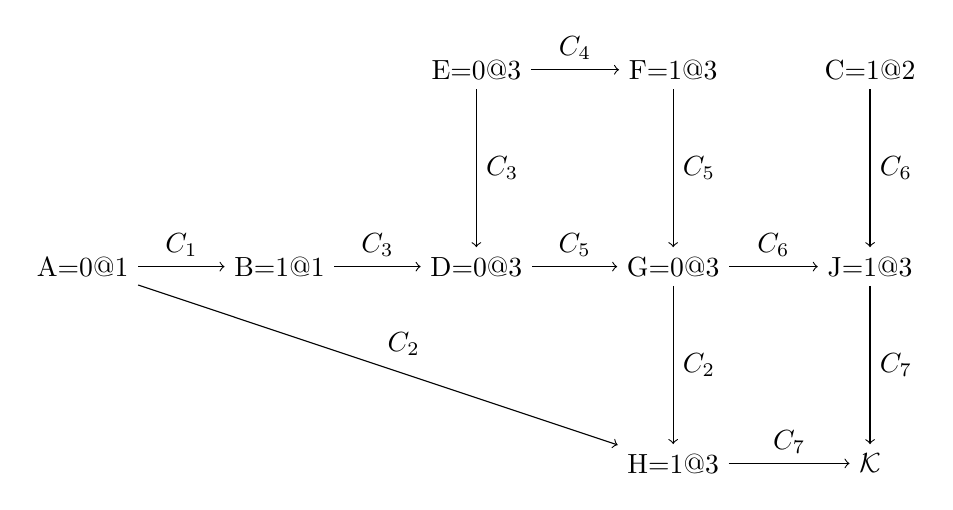
\begin{tikzpicture}[node distance=2.5cm,auto]
\node (A) {A=0@1};
\node (B) [right of=A] {B=1@1};
\node (D) [right of=B] {D=0@3};
\node (G) [right of=D] {G=0@3};
\node (H) [below of=G] {H=1@3};
\node (K) [right of=H] {$\mathcal K$};
\node (E) [above of=D] {E=0@3};
\node (F) [right of=E] {F=1@3};
\node (J) [right of=G] {J=1@3};
\node (C) [above of=J] {C=1@2};
\path[->] (G) edge node {$C_6$} (J);
\path[->] (F) edge node {$C_5$} (G);
\path[->] (C) edge node {$C_6$} (J);
\path[->] (J) edge node {$C_7$} (K);
\path[->] (E) edge node {$C_3$} (D);
\path[->] (E) edge node {$C_4$} (F);

\path[->] (A) edge node {$C_1$} (B);
\path[->] (B) edge node {$C_3$} (D);
\path[->] (D) edge node {$C_5$} (G);
\path[->] (G) edge node {$C_2$} (H);
\path[->] (H) edge node {$C_7$} (K);
\path[->] (A) edge node {$C_2$} (H);
\end{tikzpicture}%
%EndExpansion
\newline
\bigskip

  }

%\solution{
$[p]\sigma = [x:=x+y; \text{ if } x<0 \text{ then } abort \text{ else } while \text{ } x \neq y \text{ } do \text{ }... \text{ } od]\sigma 
\hspace{0.6 cm} \sigma: x \mapsto 1, y \mapsto 1\\
= [\text{if } x<0 \text{ then } abort \text{ else } while \text{ } x \neq y \text{ } do \text{ }... \text{ } od][x:=x+y]\sigma_1
\hspace{1 cm} \sigma_1: x \mapsto [x+y]\sigma = 2\\
\text{} \hspace{12 cm} y \mapsto 1\\
= [\text{if } x<0 \text{ then } abort \text{ else } while \text{ } x \neq y \text{ } do \text{ }... \text{ } od]\sigma_1
\hspace{4 cm} \underbrace{[x<0]\sigma_1=0}_{false}\\
= [\text{while } x \neq y \text{ do } x:=x+1; y:=y+2 \text{ od}]\sigma_1
\hspace{5 cm} \underbrace{[x \neq y]\sigma_1=0}_{true}\\
= [\text{while } x \neq y \text{ do } ... \text{ od}] [x:=x+1;y=y+2]\sigma_1\\
= [\text{while } x \neq y \text{ do } ... \text{ od}] [y:=y+1] [x:=x+1]\sigma_1
\hspace{3 cm} \sigma_2: x \mapsto [x+1]\sigma_1=3\\
\text{} \hspace{11.8 cm} y \mapsto 1\\
= [\text{while } x \neq y \text{ do } ... \text{ od}] [y:=y+2]\sigma_2
\hspace{4.7 cm} \sigma_3: y \mapsto [y+2]\sigma_2=3\\
\text{} \hspace{11.8 cm} x \mapsto 3\\
= [\text{while } x \neq y \text{ do } ... \text{ od}]\sigma_3
\hspace{8 cm} \underbrace{[x \neq y]\sigma_3=0}_{false}\\
= \sigma_3$
%}

\begin{exercise}{1}\label{ex:ifabort}
  Let $p$ be the following program:
  \begin{center}
  \begin{ALG}
    \ASS x{x+y};\\
    \IF\ $x<0$ \THEN\\
    \>\ABORT\\
    \ELSE\\
    \>\WHILE\ $x\neq y$ \DO\\
    \>\>\ASS x{x+1};\\
    \>\>\ASS y{y+2}\\
    \>\OD\\
    \FI
  \end{ALG}
  \end{center}
  Show that $\CA{x=2y\land y>2}p{x=y}$ is totally correct by computing the
  weakest precondition of the program.
\end{exercise}

  \solution{
The sparse method is a decision procedure for equality logic that computes
equi-satisfiable formulas in propositional logic.

Consider formula $\varphi ^{E}$ in equation logic:%

\begin{displaymath}
  \varphi ^{E}: (x_1 \neq x_2 \lor x_2=x_3 ) \land \big[ (x_2 \neq x_4 \land x_3=x_4
  \land x_4=x_5)
  \lor (x_6 \neq x_5 \land x_6=x_7 \land x_7=x_3)\big]
\end{displaymath}

Then the sets of equality literals and disequality literals of $\varphi ^{E}$
are:

\begin{eqnarray*}
E_{=}
&=&%
\{x_{2}=x_{3,}x_{3}=x_{4},x_{4}=x_{5},x_{6}=x_{7},x_{7}=x_{3}\}
\\
E_{\neq } &=&\{x_{1}\neq x_{2},x_{2}\neq x_{4},x_{6}\neq x_{5}\}
\end{eqnarray*}

It is very often the case, that a given equality logic formula $\varphi ^{E}$
can be simplified. Before reducing $\varphi ^{E}$ to a propositional formula 
$\varphi ^{P}$, we have to do some preprocessing for simplifying the
equality formula $\varphi ^{E}$:

\begin{enumerate}
\item Construct an equality graph $G^{E}(\varphi ^{E})=(V,E_{=},E_{\neq })$:

%\enlargethispage{100cm}
% Start of code
\begin{tikzpicture}[>=latex',line join=bevel,]
%%
\node (x2) at (101bp,99.026bp) [draw,circle] {$x_2$};
  \node (x3) at (149.22bp,182.55bp) [draw,circle] {$x_3$};
  \node (x1) at (14.5bp,99.026bp) [draw,circle] {$x_1$};
  \node (x6) at (293.9bp,99.026bp) [draw,circle] {$x_6$};
  \node (x7) at (245.67bp,182.55bp) [draw,circle] {$x_7$};
  \node (x4) at (149.22bp,15.5bp) [draw,circle] {$x_4$};
  \node (x5) at (245.67bp,15.5bp) [draw,circle] {$x_5$};
  \draw [solid] (x5) ..controls (262.06bp,43.885bp) and (277.41bp,70.467bp)  .. (x6);
  \definecolor{strokecol}{rgb}{0.0,0.0,0.0};
  \pgfsetstrokecolor{strokecol}
  \draw (276.75bp,53.203bp) node {$\neq$};
  \draw [solid] (x2) ..controls (117.39bp,70.641bp) and (132.74bp,44.059bp)  .. (x4);
  \draw (132.08bp,61.323bp) node {$\neq$};
  \draw [dashed] (x3) ..controls (149.22bp,136.43bp) and (149.22bp,61.789bp)  .. (x4);
  \draw (144.22bp,99.069bp) node {=};
  \draw [solid] (x1) ..controls (45.08bp,99.026bp) and (70.32bp,99.026bp)  .. (x2);
  \draw (57.714bp,107.03bp) node {$\neq$};
  \draw [dashed] (x2) ..controls (117.39bp,127.41bp) and (132.74bp,153.99bp)  .. (x3);
  \draw (132.08bp,136.73bp) node {=};
  \draw [dashed] (x6) ..controls (277.51bp,127.41bp) and (262.16bp,153.99bp)  .. (x7);
  \draw (262.82bp,136.73bp) node {=};
  \draw [dashed] (x4) ..controls (182bp,15.5bp) and (212.69bp,15.5bp)  .. (x5);
  \draw (197.38bp,7.5bp) node {=};
  \draw [dashed] (x7) ..controls (212.79bp,182.55bp) and (181.84bp,182.55bp)  .. (x3);
  \draw (197.36bp,174.55bp) node {=};
%
\end{tikzpicture}

The equality graph has two contradictory cycles, $%
c_{1}=(x_{2},x_{3},x_{4})$ and $%
c_{2}=(x_{3},x_{4},x_{5},x_{6},x_{7})$.

\item 
Following strictly the rules of the simplification algorithm, the algorithm
replace in this case every literal in the equality formula $\varphi ^{E}$
with \textsc{True}. In order to transform $\varphi ^{E}$ into a
propositional formula $\varphi ^{P}$, we have to make a little trick to
enforce the application of the reduction algorithm. In this case we apply
only one step of the simplification algorithm and replace all literals at
once with \textsc{True}, which are not in the cycles $c_{1}$ and $c_{2}$. So
we get:

\begin{eqnarray*}
\varphi _{1}^{E}:(\text{\textsc{True}}\vee \text{\textsc{True}})\wedge [
(x_{2}\,{\neq}\,x_{4}\wedge x_{3}\,{=}\,x_{4}\wedge x_{4}\,{=}
\,x_{5})\vee \\
(x_{5}\,{\neq}\,x_{6}\wedge x_{6}\,{=}\,x_{7}\wedge x_{3}\,{=}\,x_{7})]
\end{eqnarray*}

\begin{equation*}
\Rightarrow \;\;\varphi _{1}^{E}:(x_{2}\,{\neq}\,x_{4}\wedge x_{3}\,{=}\,x_{4}\wedge x_{4}\,{=}
\,x_{5})\vee \\
(x_{5}\,{\neq}\,x_{6}\wedge x_{6}\,{=}\,x_{7}\wedge x_{3}\,{=}\,x_{7})
\end{equation*}

Then the equality graph $G^{E}(\varphi _{1}^{E})$ looks like:

%\enlargethispage{100cm}
% Start of code
\begin{tikzpicture}[>=latex',line join=bevel,]
%%
\node (x2) at (14.5bp,90.939bp) [draw,circle] {$x_2$};
  \node (x3) at (206.21bp,14.5bp) [draw,circle] {$x_3$};
  \node (x6) at (206.21bp,167.38bp) [draw,circle] {$x_6$};
  \node (x7) at (261.75bp,90.939bp) [draw,circle] {$x_7$};
  \node (x4) at (116.35bp,43.697bp) [draw,circle] {$x_4$};
  \node (x5) at (116.35bp,138.18bp) [draw,circle] {$x_5$};
  \draw [solid] (x5) ..controls (147.27bp,148.23bp) and (175.43bp,157.38bp)  .. (x6);
  \definecolor{strokecol}{rgb}{0.0,0.0,0.0};
  \pgfsetstrokecolor{strokecol}
  \draw (158.33bp,161.8bp) node {$\neq$};
  \draw [solid] (x2) ..controls (47.335bp,75.709bp) and (83.51bp,58.93bp)  .. (x4);
  \draw (69.423bp,75.319bp) node {$\neq$};
  \draw [dashed] (x3) ..controls (175.19bp,24.579bp) and (146.8bp,33.804bp)  .. (x4);
  \draw (164.08bp,38.162bp) node {$=$};
  \draw [dashed] (x6) ..controls (225.32bp,141.07bp) and (242.72bp,117.12bp)  .. (x7);
  \draw (227.01bp,124.12bp) node {$=$};
  \draw [dashed] (x4) ..controls (116.35bp,76.211bp) and (116.35bp,105.82bp)  .. (x5);
  \draw (111.35bp,90.991bp) node {$=$};
  \draw [dashed] (x7) ..controls (242.64bp,64.635bp) and (225.23bp,40.683bp)  .. (x3);
  \draw (226.95bp,57.678bp) node {$=$};
%
\end{tikzpicture}

Now we have only the contradictory cycle $c_{2}$, and we can simplify the 
graph $G^{E}(\varphi _{1}^{E})$ once more by replacing all literals with TRUE, 
which are not in the cycle $c_{2}$. So we get a new equality graph 
$G^{E}(\varphi _{2}^{E})$:

\begin{tikzpicture}[>=latex',line join=bevel,]
%%
\node (x3) at (104.36bp,14.5bp) [draw,circle] {$x_3$};
  \node (x6) at (104.36bp,167.38bp) [draw,circle] {$x_6$};
  \node (x7) at (159.9bp,90.939bp) [draw,circle] {$x_7$};
  \node (x4) at (14.5bp,43.697bp) [draw,circle] {$x_4$};
  \node (x5) at (14.5bp,138.18bp) [draw,circle] {$x_5$};
  \draw [solid] (x5) ..controls (45.422bp,148.23bp) and (73.58bp,157.38bp)  .. (x6);
  \definecolor{strokecol}{rgb}{0.0,0.0,0.0};
  \pgfsetstrokecolor{strokecol}
  \draw (56.479bp,161.8bp) node {$\neq$};
  \draw [dashed] (x4) ..controls (14.5bp,76.211bp) and (14.5bp,105.82bp)  .. (x5);
  \draw (9.5bp,90.991bp) node {$=$};
  \draw [dashed] (x3) ..controls (73.438bp,24.547bp) and (45.28bp,33.696bp)  .. (x4);
  \draw (62.381bp,38.115bp) node {$=$};
  \draw [dashed] (x6) ..controls (123.47bp,141.07bp) and (140.87bp,117.12bp)  .. (x7);
  \draw (125.16bp,124.12bp) node {$=$};
  \draw [dashed] (x7) ..controls (140.79bp,64.635bp) and (123.38bp,40.683bp)  .. (x3);
  \draw (125.1bp,57.678bp) node {$=$};
%
\end{tikzpicture}

Recall the theorem,%
\begin{equation*}
\varphi ^{E}\text{ is satisfiable }\Leftrightarrow e(\varphi ^{E})\AND B_{t}%
\text{ is satisfiable,}
\end{equation*}

where $e(\varphi ^{E})$ denotes the \textit{propositional skeleton} of $%
\varphi ^{E}$and $B_{t}$ is a formula that describes the \textit{%
transitivity constraints} (conjunctions of implications).

So $\varphi ^{P}=e(\varphi ^{E})\AND B_{t}$ is equi-satisfiable to $\varphi
^{E}$, iff $\varphi ^{E}$ is satisfiable.

\bigskip
\item First we construct the propositional skeleton of $\varphi _{2}^{E}$ by
replacing each atom of the form $x_{i}=x_{j}$ in $\varphi _{2}^{E}$ with $%
e_{i,j}$, such that:%
\begin{equation*}
e(\varphi _{2}^{E})=(e_{3,4}\AND e_{4,5})\OR(\lnot e_{5,6}\AND e_{1,6} \AND 
e_{3,7})
\end{equation*}

\item Construct the nonpolar equality graph $G_{NP}^{E}(\varphi _{2}^{E})$:

\begin{tikzpicture}[>=latex',line join=bevel,]
%%
\node (x3) at (104.36bp,14.5bp) [draw,circle] {$x_3$};
  \node (x6) at (104.36bp,167.38bp) [draw,circle] {$x_6$};
  \node (x7) at (159.9bp,90.939bp) [draw,circle] {$x_7$};
  \node (x4) at (14.5bp,43.697bp) [draw,circle] {$x_4$};
  \node (x5) at (14.5bp,138.18bp) [draw,circle] {$x_5$};
  \draw [solid] (x5) ..controls (45.422bp,148.23bp) and (73.58bp,157.38bp)  .. (x6);
  \draw [solid] (x4) ..controls (14.5bp,76.211bp) and (14.5bp,105.82bp)  .. (x5);
  \draw [solid] (x3) ..controls (73.438bp,24.547bp) and (45.28bp,33.696bp)  .. (x4);
  \draw [solid] (x6) ..controls (123.47bp,141.07bp) and (140.87bp,117.12bp)  .. (x7);
  \draw [solid] (x7) ..controls (140.79bp,64.635bp) and (123.38bp,40.683bp)  .. (x3);
%
\end{tikzpicture}

\item Make $G_{NP}^{E}(\varphi _{2}^{E})$ chordal, using elimination
ordering $(x_{3},x_{4},x_{5},x_{6},x_{7})$:

\begin{tikzpicture}[>=latex',line join=bevel,]
%%
\node (x3) at (104.36bp,14.5bp) [draw,circle] {$x_3$};
  \node (x6) at (104.36bp,167.38bp) [draw,circle] {$x_6$};
  \node (x7) at (159.9bp,90.939bp) [draw,circle] {$x_7$};
  \node (x4) at (14.5bp,43.697bp) [draw,circle] {$x_4$};
  \node (x5) at (14.5bp,138.18bp) [draw,circle] {$x_5$};
  \draw [solid] (x5) ..controls (44.939bp,148.07bp) and (73.303bp,157.29bp)  .. (x6);
  \draw [solid] (x5) ..controls (55.749bp,124.78bp) and (117.74bp,104.64bp)  .. (x7);
  \draw [solid] (x3) ..controls (73.438bp,24.547bp) and (45.28bp,33.696bp)  .. (x4);
  \draw [solid] (x3) ..controls (78.612bp,49.939bp) and (40.44bp,102.48bp)  .. (x5);
  \draw [solid] (x6) ..controls (123.47bp,141.07bp) and (140.87bp,117.12bp)  .. (x7);
  \draw [solid] (x4) ..controls (14.5bp,76.211bp) and (14.5bp,105.82bp)  .. (x5);
  \draw [solid] (x7) ..controls (140.79bp,64.635bp) and (123.38bp,40.683bp)  .. (x3);
%
\end{tikzpicture}

\item Generate the transitivity constraints in $B_{t}$ for every triangle in
the chordal graph $G_{NP}^{E}(\varphi _{2}^{E})$:

\begin{enumerate}
\item $B_{t}=$ \textsc{True}

\item For each triangle $(e_{i,j},e_{j,k},e_{i,k})$ in $G_{NP}^{E}(\varphi
_{2}^{E})$:%
\begin{eqnarray*}
B_{t}=((e_{3,4}\AND e_{4,5}\IMPL e_{3,5})\AND && \\
(e_{3,5}\AND e_{4,5}\IMPL e_{3,4})\AND && \\
(e_{3,4}\AND e_{3,5}\IMPL e_{4,5})\AND && \\
(e_{3,5}\AND e_{5,7}\IMPL e_{3,7})\AND && \\
(e_{3,7}\AND e_{3,5}\IMPL e_{5,7})\AND && \\
(e_{3,7}\AND e_{5,7}\IMPL e_{3,5})\AND && \\
(e_{5,6}\AND e_{6,7}\IMPL e_{5,7})\AND && \\
(e_{6,7}\AND e_{5,7}\IMPL e_{5,6})\AND && \\
(e_{5,6}\AND e_{5,7}\IMPL e_{6,7})) &&
\end{eqnarray*}

Hence, $\varphi ^{E}$ is satisfiable, iff $\varphi ^{P}=e(\varphi _{2}^{E})%
\AND B_{t}$ is satisfiable.
\end{enumerate}
\end{enumerate}


  }


\begin{exercise}{1}
  Let $p$ be the program given in exercise~\ref{ex:ifabort}.
  Use the Hoare calculus to show that
  \[\CA{x=2y\land y>2}p{x=y}\]
  is totally correct.
\end{exercise}

\documentclass[a4paper,parskip=half]{scrartcl}
%%%%%%%%%%%%%%%%%%%%%%%%%%%%%%%%%%%%%%%%%%%%%%%%%%%%%%%%%%%%%%%%%%%%%%%%%%%%%%%%%%%%%%%%%%%%%%%%%%%%%%%%%%%%%%%%%%%%%%%%%%%%%%%%%%%%%%%%%%%%%%%%%%%%%%%%%%%%%%%%%%%%%%%%%%%%%%%%%%%%%%%%%%%%%%%%%%%%%%%%%%%%%%%%%%%%%%%%%%%%%%%%%%%%%%%%%%%%%%%%%%%%%%%%%%%%
\usepackage{eurosym}
\usepackage[utf8]{inputenc}
\usepackage[T1]{fontenc}
\usepackage{lmodern}
\usepackage[english]{babel}
\usepackage{graphicx}
\usepackage{scrpage2}
\usepackage{ifthen}
\usepackage[ruled, boxed]{algorithm2e}
\usepackage{amsmath}
\usepackage{amsthm}
\usepackage{amssymb}
\usepackage{units}
\usepackage{enumerate}

\setcounter{MaxMatrixCols}{10}
%TCIDATA{OutputFilter=Latex.dll}
%TCIDATA{Version=5.00.0.2606}
%TCIDATA{<META NAME="SaveForMode" CONTENT="1">}
%TCIDATA{BibliographyScheme=Manual}
%TCIDATA{LastRevised=Friday, April 01, 2011 07:06:22}
%TCIDATA{<META NAME="GraphicsSave" CONTENT="32">}

\newcounter{exercise}
\setcounter{exercise}{1}
\newenvironment{exercise}[1]{\large \textsf{\textbf{Problem \arabic{exercise}}} \ifthenelse{#1>0}{(#1 points)}{} \\ \normalsize \addtocounter{exercise}{1}}{\vspace{2ex}}
\newenvironment{solution}{\large \textsf{\textbf{Solution:}} \\ \normalsize}{\vspace{2ex}}
\newenvironment{remark}{\large \textsf{\textbf{Remark}} \\ \normalsize}{\vspace{2ex}}
\newtheorem{claim}{Claim}
\newtheorem{lemma}{Lemma}
\input{tcilatex}

\begin{document}


\thispagestyle{scrheadings} ~

\subsection{solution}
\hfill \newline
At first we have to check if \textbf{Set-Partition} is a membership of NP.%
\newline
This can be shown by using a simple guess \& check procedure:\newline

Guess an arbitrary subset $S_1\subseteq S$ and verify if the sum of the
elements in $S_1$ and in $S\backslash S_1$ are equal. The summing of the
elements in the subsets takes linear time in the size of $S$.

To show NP-hardness of \textbf{Set-Partition}, we reduce \textbf{%
Subset-Sum} to \textbf{Set-Partition}.

Let $S=\{b_{1},\ldots ,b_{n}\}$ be a set of integers and an integer $t$ be a target. Let $S^{\prime }$ be an instance of 
\textbf{Set-Partition}, such that $S^{\prime }=S\cup \{c\}$ with $c=M-2\cdot
t$ and $M=\tsum\limits_{i\in S}b_{i}$.

We have to show following equation:%
\begin{equation*}
(S,t)\in 
%TCIMACRO{\TeXButton{Subset-Sum}{\mbox{\textbf{Subset-Sum}}}}%
%BeginExpansion
\mbox{\textbf{Subset-Sum}}%
%EndExpansion
\Leftrightarrow S^{\prime }\in 
%TCIMACRO{\TeXButton{Set-Partition}{\mbox{\textbf{Set-Partition}}}}%
%BeginExpansion
\mbox{\textbf{Set-Partition}}%
%EndExpansion
\end{equation*}

\begin{proof}
\hfill\newline
$\Leftarrow :$ Suppose that $S^{\prime }=\{b_{1},\ldots ,b_{n+1}\}$ is a
positive instance of \textbf{Set-Partition}. Then there exists a subset $%
S_1\subseteq S^{\prime }$,which specify the partition, such that $S_2=S^{\prime
}\backslash S_1$ and the sum of the elements in\ $S_1$ and $S_2$ are equal.

Let $S^1=\tsum\limits_{i\in S_1}b_{i}$ and $S^2=\tsum\limits_{i\in B}b_{i}$
be the sum of the elements in the subsets. Since $c=M-2\cdot t$ and $c\in
S^{\prime }$, hence $c$ is in one of the two partitions.

Without loss of generality, suppose that $c\in S_1$. Then $N=M+c=M+M-2\cdot
t=2\cdot M-2\cdot t=\tsum\limits_{i\in S^{\prime }}b_{i}$. Since $S^1=S^2
$ and $N=S^1+S^2$, it follows that $S^1=S^2=\frac{N}{2}=$ $\frac{%
2\cdot M-2\cdot t}{2}=M-t$.

Since $c\in S_1$ and $c=M-2\cdot t$, we can conclude that $S^1=t+c$. If $c$
is in the fist part of the partition, then $S_1\backslash \{c\}$ is a subset
of $S$ that sum to $t$, and if $c$ is in the second part of the partition,
then $S_2\backslash \{c\}$ is a subset of elements of $S$ that sum to $t$.
Hence, $(S,t)$ is a positive instance of \textbf{Subset-Sum}.

$\Rightarrow :$ Suppose that $(S,t)$ is a positive instance of \textbf{%
Subset-Sum}. Then there exists a subset $T\subseteq S$ such that $%
\tsum\limits_{i\in T}b_{i}=t$.

We have to show that $S^{\prime }=S\cup \{c\}$ is a positive instance of 
\textbf{Set-Partition}. Thus, we have to find two subsets of $S^{\prime }$
such that $S^1=S^2$. This can be done easily by setting $S_1=T\cup \{c\}$.
Then $S^1=t+M-2\cdot t=M-t=\frac{N}{2}$, wich is exactly the half of the
sum of elements in $S^{\prime }$, i.e. $S^1=\frac{N}{2}=S^2$. This
implies that $S^{\prime }$ is partitionable. Thus, $S^{\prime }$ is a
positive instance of \textbf{Set-Partition}.
\end{proof}

Since \textbf{Set-Partition} $\in $ NP and is NP-hard, it follows that it is
NP-complete.
\end{solution}

\begin{remark}
To see how algorithms are represented in pseudo-code see how algorithms are
described in the book \^{a}\euro \oe Introduction to Algorithms\^{a}\euro 
\"{\i}\textquestiondown 
%TCIMACRO{\U{bd} }%
%BeginExpansion
$\frac12$
%EndExpansion
by Cormen, Leiserson, Rivest, and Stein. A link to the book (that let\^{a}%
\euro \texttrademark s you browse the pages of the book) can be found on
Moodle.

Also recall the $\mathcal{O}$-notation: Let $f$ and $g$ be two functions
from the natural numbers onto the positive real numbers. If there exist
constants $c>0$ and $n_{0}\geq 0$ such that for all $n\geq n_{0}$, $f(n)\leq
c\cdot g(n)$, then we write $f(n)=\mathcal{O}(g(n))$. Let $n$ be the size of
the cost matrix of a finite game. The running time $T(n)$ of an algorithm
takes time polynomial in $n$, if there exists an integer constant $d>0$ such
that $T(n)=\mathcal{O}(n^{d})$. For more details see Chapter 3 in the above
book.
\end{remark}

\end{document}



\begin{exercise}{1}
  Extend our toy language by statements of the form ``$\kw{assert}\
  e$''. When the condition~$e$ evaluates to true, the program
  continues, otherwise the program aborts.

  Specify the syntax and semantics of the extended language.
  Determine the weakest precondition, the weakest liberal
  precondition, the strongest postcondition, and Hoare rules
  (partial and total correctness) for \kw{assert}-statements.
  Show that they are correct.

  Treat the \kw{assert}-statement as a first-class citizen, i.e., do
  not refer to other program statements in the final result.  However,
  you may use other statements as intermediate steps when deriving the
  rules.
\end{exercise}

\begin{solution}

test

\end{solution}

\begin{exercise}{1}
  Verify that the following program doubles the value of~$x$.
  For which inputs does it terminate? Choose appropriate pre-
  and postconditions and show that the assertion is totally correct.
  Use $y=2x_0+x$ as a starting point for the invariant,
  where $x_0$ denotes the initial value of~$x$.
\begin{center}
  \begin{ALG}
    \ASS y{3x};\\
    \WHILE\ $2x\neq y$\ \DO\\
    \>\ASS x{x+1};\\
    \>\ASS y{y+1};\\
    \OD
  \end{ALG}
\end{center}    
\end{exercise}

%\solution{
\textbf{Solution:}\newline
\\
\noindent We have choosen the following\\
Precondition$:= x=x_0 \land x \ge 0$ and\\
Postcondition$:= x=2x_0$ and\\
extended the Invariant$:= 2x_0+x=y \land x \ge 0$\\

\bigskip
\noindent Now we want to show the assertion is totally correct:\\
\\
\begin{ALG}
\ASSERTN1{\text{Precondtion: } x=x_0 \land x \ge 0}\\
\ASSERTN4{\INV \sub{y<-3x}}	\quad(as)$\ua$\\
$y \leftarrow 3x;$\\
\ASSERTN3{\INV := 2x_0+x=y \land x \ge 0}	\quad(wht'')\\
\WHILE\ $2x \neq y$ \DO\\
\ASSERTN9{\INV \land 2x \neq y \land t=t_0}	\quad(wht'')\\
\ASSERTN8{\INV \land 0 \le t < t_0 \sub{y<-y+1} \sub{x<-x+1}} 
\quad(as)$\ua$\\
\>\ $x \leftarrow x+1;$\\
\ASSERTN7{\INV \land 0 \le t < t_0 \sub{y<-y+1}}	
\quad(as)$\ua$\\
\>\ $y \leftarrow y+1;$\\
\ASSERTN6{\INV \land 0 \le t < t_0}	\quad(wht'')\\
\OD\\
\ASSERTN5{\INV \land 2x = y}	\quad(wht'')\\
\ASSERTN2{\text{Postcondition: } x=2x_0}
\end{ALG}

\bigskip
\noindent We define the bound function $t$ as:\\
$t:=y-2x$,\\
which fulfils the criteria for bound functions (listed in exercise 7).\\

\bigskip
\noindent Now the implications:\\�
\\
\textbf{$1 \rightarrow 4:$}\\
\indent $x=x_0 \land x \ge 0 \rightarrow Inv [y|3x]$\\
$= x=x_0 \land x \ge 0 \rightarrow 2x_0+x = y \land x \ge 0 [y|3x]$\\
$= \textcolor{green}{x=x_0} \land x \ge 0 \rightarrow \textcolor{green}{\underbrace{2x_0}_{=2x}}+x = 3x \land x \ge 0$\\
$= x=x_0 \land x \ge 0 \rightarrow \underbrace{3x = 3x}_{true} \checkmark\\
\indent \land x \ge 0$\\
$= x=x_0 \land \textcolor{magenta}{x \ge 0} \rightarrow \underbrace{3x = 3x}_{true} \checkmark\\
\indent \land \textcolor{magenta}{x \ge 0} \checkmark$\\
\\
\textbf{$5 \rightarrow 6:$}\\
\indent $Inv \land 2x \neq y \land t = t_0 \rightarrow Inv \land 0 \le t < t_0 [y|y+1] [x|x+1]$\\
$= 2x_0+x = y \land x \ge 0 \land 2x \neq y \land t = t_0\\ 
\indent \rightarrow 2x_0+x = y \land x \ge 0 \land 0 \le t < t_0 [y|y+1] [x|x+1]$\\
$= 2x_0+x = y \land x \ge 0 \land 2x \neq y \land t = t_0\\ 
\indent \rightarrow 2x_0+x+1 = y+1 \land x+1 \ge 0 \land 0 \le t < t_0$\\
$= 2x_0+x = y \land x \ge 0 \land 2x \neq y \land t = t_0\\ 
\indent \rightarrow 2x_0+x+1 = y+1 \land x+1 \ge 0 \land 0 \le \underbrace{\underbrace{t}_{=y+1-2(x+1)}}_{=y-2x-1} < \underbrace{t_0}_{=y-2x}$\\
$= 2x_0+x = y \land x \ge 0 \land 2x \neq y \land t = t_0\\ 
\indent \rightarrow 2x_0+x+1 = y+1 \land x+1 \ge 0 \land \underbrace{0 \le y-2x-1 < y-2x}_{true}$\\
$= 2x_0+x = y \land x \ge 0 \land 2x \neq y \land t = t_0\\ 
\indent \rightarrow 2x_0+x$ \sout{$+1$} $= y$ \sout{$+1$} $\land x+1 \ge 0 \land \underbrace{0 \le y-2x-1 < y-2x}_{true}$\\
$= \textcolor{green}{2x_0+x = y} \land x \ge 0 \land 2x \neq y \land t = t_0\\ 
\indent \rightarrow \textcolor{green}{2x_0+x = y} \checkmark \\
\indent \land x+1 \ge 0\\ 
\indent \land 0 \le y-2x-1 < y-2x \checkmark$\\
$= 2x_0+x = y \land \textcolor{magenta}{x \ge 0} \land 2x \neq y \land t = t_0\\ 
\indent \rightarrow 2x_0+x = y \checkmark \\
\indent \land \textcolor{magenta}{\underbrace{x+1 \ge 0}_{=x \ge -1}} \checkmark \\ 
\indent \land 0 \le y-2x-1 < y-2x \checkmark$\\
\\
\textbf{$9 \rightarrow 2:$}\\
\indent $Inv \land 2x = y \rightarrow x = 2x_0$\\
$= \textcolor{green}{2x_0+x = \underbrace{y}_{=2x}} \land x \ge 0 \land \textcolor{green}{2x = y} \rightarrow x = 2x_0$\\
$= 2x_0$ \sout{$+x$} $=$ \sout{$2$} $x \land x \ge 0 \land 2x = y \rightarrow x = 2x_0$\\
$= \textcolor{magenta}{2x_0 = x} \land x \ge 0 \land 2x = y \rightarrow \textcolor{magenta}{x = 2x_0} \checkmark$\\
\\
So the correctness asertion above is totally correct.\\
It terminates for all integers $(x_0)$ which are greater or equal 0.
%}

\begin{exercise}{1}
    Show that the following correctness assertion is totally correct.
    Describe the function computed by the program if we consider $a$
    as its input and $c$ as its output.
\begin{center}
  \begin{ALG}
    \ASSERTN1{a\geq0}\\
    \ASS b1;\\
    \ASS c0;\\
    \ASSERTN\INV{b=(c+1)^3\land 0\leq c^3\leq a}\\
    \WHILE\ $b\leq a$\ \DO\\
    \>\ASS d{3*c+6};\\
    \>\ASS c{c+1};\\
    \>\ASS b{b+c*d+1}\\
    \OD\\
    \ASSERTN2{c^3\leq a<(c+1)^3}
  \end{ALG}
\end{center}    
\end{exercise}

\subsection{solution}

\subsubsection{Algorithm}
\begin{algorithmic}
\Function{DFS}{$a$}
    \For {each vertex $u \in V[G]$}
        \State color[u] $\gets$ k
        \State $\pi[u] \gets NULL$
    \EndFor \\
    \State $time \gets 0$
\EndFunction
\end{algorithmic}

\smallskip

\begin{algorithmic}
\Function{DFS-Visit}{$u$}
    \State color[u] $\gets$ k
    \State d[u] $\gets$ time $\gets$ time + 1
    \For {each $v \in Adj[u]$}
      \State $\triangleright$ explore edge $(u,v)$
      \If {color[v] = k}
          \State $\pi[v] \gets u$
          \State DFS-Visit($v$)
      \EndIf
    \EndFor
    \State color[v] $\gets$  k
    \State f[u] $\gets$ time $\gets$ time + 1
\EndFunction
\end{algorithmic}

\subsubsection{Description}
The definition of the tree saies that:
\begin{itemize}
 \item there are no cycles allowed
 \item paths are connected
\end{itemize}


\begin{exercise}{1}
  Prove that the rule
\[
\begin{array}{c}
\WH{\CA{\INV}{\WHILE\ e\ \DO\ p\ \OD}{\INV\land\lnot e}}%
   {\CA{\INV\land e}{p}{\INV}}
\end{array}
\]
is correct regarding partial correctness, i.e., show that
$\CA{\INV}{\WHILE\ e\ \DO\ p\ \OD}{\INV\land\lnot e}$ is partially correct
whenever $\CA{\INV\land e}{p}{\INV}$ is partially correct.
\end{exercise}

\textbf{Solution:}\newline

To prove the $\kw{while}$-rule for partial correctnes we have to consider
following definition: 
\begin{definition}
	Let $\{F\}\, p\, \{G\}$ be an arbitrary partial correctness assertion. Then $\{F\}\, p\, \{G\}$ is
	sound if
	\begin{equation*}
		\vdash_{par} \{F\}\, p\, \{G\}\quad \text{ then } \vDash_{par} \{F\}\, p\, \{G\}.
	\end{equation*}
\end{definition}

Then let $I$ be an arbitrary interpretation and assume that $\vDash _{%
\mathrm{par}}^{I}\{\mathrm{Inv}\,\wedge \,e\}\,p\,\{\mathrm{Inv}\}$, i.e. is
partially correct. Then for some fixed state $\tau $ which satisfies the
invariant $\mathrm{Inv}$ and $e$ in the precondition, there $\exists \tau
^{\prime }\in \mathcal{S}$ such that $[p]\tau =\tau ^{\prime }$ is defined
and $\tau ^{\prime }$ satisfies $\mathrm{Inv}$ in the postcondition. To
prove that $\vDash _{\mathrm{par}}^{I}\{\mathrm{Inv}\}\,\kw{while}\ e\ %
\kw{do}\ p\ \kw{od}\,\{\mathrm{Inv}\,\wedge \,\lnot e\}$ is valid, we have
to show for all states $\sigma \in \mathcal{S}$, such that%
\begin{equation*}
\mathrm{Inv}\,\Rightarrow \,F\quad \lbrack F]\sigma \text{ is true, then }[%
\kw{while}\ e\ \kw{do}\ p\ \kw{od}]\sigma \text{ is true with }%
G\,\Rightarrow \,(\mathrm{Inv}\,\wedge \,\lnot e).
\end{equation*}

The proof can be done by using structural induction on the given axiom rule.

We shall show by induction that $P(n),n\in \mathbb{N}$ holds, where%
\begin{eqnarray*}
P(n)\quad \overset{defined}{\Longleftrightarrow }\quad \forall \sigma
,\sigma ^{\prime \prime } &\in &\mathcal{S}\text{ such that }(\sigma ,\sigma
^{\prime \prime })\in \Theta _{n}\text{ and} \\
\sigma &\vDash &_{\mathrm{par}}^{I}\mathrm{Inv}\;\Rightarrow \;\sigma
^{\prime \prime }\vDash _{\mathrm{par}}^{I}(\in \mathcal{S}),
\end{eqnarray*}

for all $n$ iteration-steps of $\kw{while}\ e\ \kw{do}\ p\ \kw{od}$. ( $%
(\sigma ,\sigma ^{\prime \prime })\in \Theta _{n}$ denotes a partial
function.)

\bigskip

\textit{Base case:}

If $n=0$, then the induction hypothesis $P(0)$ is vacuosly true.

\bigskip

\textit{Induction step:}

We assume that the induction hypothesis $P(n)$ for $n\geq 0$ holds and try
to prove $P(n+1)$.

Let $w\equiv \kw{while}\ e\ \kw{do}\ p\ \kw{od}$, and consider some
arbitrary states $\sigma ,\sigma ^{\prime },\sigma ^{\prime \prime }\in 
\mathcal{S}$ with $[\mathrm{Inv}]\sigma =true$ (in the precondition).

We have to show that $\sigma ^{\prime \prime }\vDash _{\mathrm{par}}^{I}(%
\mathrm{Inv}\,\wedge \,\lnot e)$, i.e. $[\mathrm{Inv}\,\wedge \,\lnot
e]\sigma ^{\prime \prime }=true$. Then there are existing two cases for any $%
\tau \in \mathcal{S}$:

\bigskip

\begin{description}
\item[\textbf{case} \textit{i)}] $[e]\tau =true$. Since by assumption $%
\vDash _{\mathrm{par}}^{I}\{\mathrm{Inv}\,\wedge \,e\}\,p\,\{\mathrm{Inv}\}$
is partially correct, i.e.%
\begin{eqnarray*}
\forall \sigma  &\in &\mathcal{S}, \\
&&\text{if }[\mathrm{Inv}\,\wedge \,e]\sigma =true\;\Rightarrow \;[p]\sigma 
\text{ is defined and }[\mathrm{Inv}][p]\sigma =true.
\end{eqnarray*}

\item Then we have $\sigma \vDash _{\mathrm{par}}^{I}e$ and hence $\sigma
\vDash _{\mathrm{par}}^{I}(\mathrm{Inv}\,\wedge \,e)$.

\item Thus,%
\begin{equation*}
(w,\sigma )\,\Rightarrow \,(p;w,\sigma )\,\Rightarrow ^{\ast }\,\sigma
^{\prime \prime }.
\end{equation*}

\item Hence, $[w]\sigma =\sigma ^{\prime \prime }$ is defined and satisfies $%
\mathrm{Inv}$ in the postcondition.

\item From the induction hypothesis $P(n)$ we obtain $\sigma ^{\prime \prime
}\vDash _{\mathrm{par}}^{I}(\mathrm{Inv}\,\wedge \,\lnot e)$, since for $%
[e]\sigma \neq 0$,%
\begin{equation*}
(p,\sigma )\,\Rightarrow \,\sigma ^{\prime }\quad \text{and\quad }(w,\sigma
^{\prime })\,\Rightarrow ^{\ast }\,\sigma ^{\prime \prime }.\,
\end{equation*}

\item Since $[\mathrm{Inv}\,\wedge \,e]\sigma =true$, $[p]\sigma $ is
defined and we obtain $\sigma ^{\prime }\vDash _{\mathrm{par}}^{I}\mathrm{Inv%
}$, as $\vDash \{\mathrm{Inv}\,\wedge \,\lnot e\}\,p\,\{\mathrm{Inv}\}$.

\item Then the induction hypothesis can be applied to $[w]\sigma ^{\prime
}=\sigma ^{\prime \prime }$ which gives us $[\mathrm{Inv}\,\wedge \,\lnot
e]\sigma ^{\prime \prime }=true$.

\item[\textbf{case} \textit{ii)}] $[e]\tau =false$. Then we have $\sigma
\vDash _{\mathrm{par}}^{I}\lnot e$ and \ hence $\sigma \vDash _{\mathrm{par}%
}^{I}(\mathrm{Inv}\,\wedge \,\lnot e)$, i.e. $[\mathrm{Inv}\,\wedge \,\lnot
e]\sigma =true$. Then according to%
\begin{equation*}
(w,\sigma ^{\prime \prime })\,\Rightarrow \,\sigma \quad \text{if }[e]\sigma
^{\prime \prime }=0,
\end{equation*}

\item i.e. $[w]\sigma ^{\prime \prime }=\sigma $. This establishes the
induction hypothesis $P(n+1)$.$\quad \Rightarrow \,P(n)$ holds for all $n$
and the rule for $\kw{while}$ is \textit{sound}.

\item 
\end{description}



\begin{exercise}{2}
  Determine the weakest liberal precondition of \WHILE-loops, i.e.,
  find a formula equivalent to $\WLP(\WHILE\ e\ \DO\ p\ \OD, G)$
  similar to the weakest precondition in the course.

  Use your formula to compute the weakest liberal precondition of
  the program 
  \begin{center}
     \ASS z0;
     \WHILE\ $y\neq0$ \DO
       \ASS z{z+x};
       \ASS y{y-1}
     \OD
  \end{center}
  with respect to the postcondition $z=x*y_0$. Compare the result
  to the weakest precondition computed in the course and explain
  the differences.
\end{exercise}

\subsection{solution}
This can be explained by using a small procedure (see Procedure \ref%
{Alg-N-Sorted-El}) for this problem.

%TCIMACRO{%
%\TeXButton{Algorithm: N-SORTED-ELEMENTS}{\floatname{algorithm}{Procedure}
%\renewcommand{\algorithmicrequire}{\textbf{Input:}}
%\renewcommand{\algorithmicensure}{\textbf{Output:}}
%\renewcommand{\algorithmicforall}{\textbf{for each}}
%
%\begin{algorithm}[ht]
%\small
%\begin{algorithmic}
%	\Require $L=(e_{1},\ldots , e_{n}), k\in \mathbb{N}^{+}$
%	\Ensure $\mathbf{true}$ if $n$-sorted elements of size $k$ are found, $\mathbf{false}$ otherwise.
%	\newline
%	\State $i \leftarrow 1$
%	\State $count \leftarrow 1$ \Comment{count variable for finding $n$-sorted elements of size $k$.} 
%	\ForAll{$i \;$ s.t. $\; 1 \leq i \leq |L| - 1$}
%		\If{$\left(e(i) + 1\right) = e(i+1)$}
%			\State $count \leftarrow count + 1$
%		\Else
%			\If{$count = k$}
%				\Return \textbf{true}
%			\Else
%				\State $count \leftarrow 1$ \Comment{the number of sorted elements was $< k$; $\Rightarrow$ reset the count value.}
%			\EndIf
%		\EndIf
%	\EndFor\\
%	\Return \textbf{false}	
%\end{algorithmic}
%\caption{\small \textsc{N-Sorted-Elements} procedure.}
%\label{Alg-N-Sorted-El}
%\end{algorithm}}}%
%BeginExpansion
\floatname{algorithm}{Procedure}
\renewcommand{\algorithmicrequire}{\textbf{Input:}}
\renewcommand{\algorithmicensure}{\textbf{Output:}}
\renewcommand{\algorithmicforall}{\textbf{for each}}

\begin{algorithm}[ht]
\small
\begin{algorithmic}
	\Require $L=(e_{1},\ldots , e_{n}), k\in \mathbb{N}^{+}$
	\Ensure $\mathbf{true}$ if $n$-sorted elements of size $k$ are found, $\mathbf{false}$ otherwise.
	\newline
	\State $i \leftarrow 1$
	\State $count \leftarrow 1$ \Comment{count variable for finding $n$-sorted elements of size $k$.} 
	\ForAll{$i \;$ s.t. $\; 1 \leq i \leq |L| - 1$}
		\If{$\left(e(i) + 1\right) = e(i+1)$}
			\State $count \leftarrow count + 1$
		\Else
			\If{$count = k$}
				\Return \textbf{true}
			\Else
				\State $count \leftarrow 1$ \Comment{the number of sorted elements was $< k$; $\Rightarrow$ reset the count value.}
			\EndIf
		\EndIf
	\EndFor\\
	\Return \textbf{false}	
\end{algorithmic}
\caption{\small \textsc{N-Sorted-Elements} procedure.}
\label{Alg-N-Sorted-El}
\end{algorithm}%
%EndExpansion

The above procedure can be solved in logarithmic space in the size of the
input $I$ with $|I|=|L|$.\newline
\noindent The procedure needs only one pointer to an element in the list $L$
and one count variable of constant size. I.e. the pointer variable $i$ need $%
\log (n) $ bits for its representation. Observe a very large list $L$ of
non-negative intergers. Since the memory of a program is limited to constant
many pointers, the pointer variable $i$ uses at most $O(\log _{2}|L|)$ bits
of memory.

\bigskip


%%TCIMACRO{%
%%\TeXButton{algorithm: N-SORTED-ELEMENTS}{\begin{algorithm}
%%	\KwIn{non-empty list L, integer k $\geq$ 1}
%%	\KwOut{bool}
%%		int count $\leftarrow 1;$\\
%%		\For{i in 1 \KwTo n}{
%%			\If{$L[i]==L[i+1]$}{
%%				$count = count+1;$\\ }
%%			\Else {
%%				\If{$count==k$}
%%					return ("yes");\\ 
%%				\Else 
%%					\tcc{number of sorted elements was too small}
%%					$count = 1$;\\
%%				\ Fi
%%			}
%%		}
%%		return ("no");
%%	\caption{\textfb{N-SORTED-ELEMENTS}}
%%	\label{alg:n-sorted}
%%\end{algorithm}}}%
%%BeginExpansion
%\begin{algorithm}[H]
%	\KwIn{non-empty list L, integer k $\geq$ 1}
%	\KwOut{bool}
%		int count $\leftarrow 1;$\\
%		\For{i in 1 \KwTo n} {
% 			\If{$L[i]==L[i+1]$}{
%				$count = count+1;$\\ }
%			\Else {
%				\If{$count==k$}
%					{return ("yes");\\ }
%				\Else 
%					{\tcc{number of sorted elements was too small}
%					$count = 1$;\\}
%			}
%		}
%		return ("no")
%% 	\caption{\textfb{N-SORTED-ELEMENTS}}
%	\label{alg:n-sorted}
%\end{algorithm}%
%%EndExpansion
%
%The algorithm above requires logarithmic space in the sice of the length of the input list:\\
%\newline
%\begin{itemize}
% \item $ count needs log_2|n| space.$
%\end{itemize}


\end{document}
